\documentclass[a4paper,11pt] {article}
% Default margins are too wide all the way around. I reset them here
\setlength{\topmargin}{.5in}
\setlength{\textheight}{9in}
\setlength{\oddsidemargin}{.125in}
\setlength{\textwidth}{6.25in}

\usepackage{color}
\usepackage[utf8]{inputenc}
\usepackage{graphicx}
\usepackage{float}
\usepackage{pdfpages}
\usepackage{amsthm}
\usepackage{amsmath,amsfonts,amssymb,amsthm}
\usepackage{url}
\usepackage{hyperref}
\usepackage{pdfpages}
\theoremstyle{definition}
\newtheorem{defn}{Definition}[section]
\newtheorem{conj}{Conjecture}[section]
\newtheorem{exmp}{Example}[section]

\definecolor{javared}{rgb}{0.6,0,0} % for strings
\definecolor{javagreen}{rgb}{0.25,0.5,0.35} % comments
\definecolor{javapurple}{rgb}{0.5,0,0.35} % keywords
\definecolor{javadocblue}{rgb}{0.25,0.35,0.75} % javadoc
%\usepackage[french]{babel}
\usepackage[T1]{fontenc}


\begin{document}
\title{\textbf{Usability of touch-based devices \\ Skeuomorph and Flat design}}
\author{\textbf{Bodart Xavier} - \textbf{Chapeaux Thomas} - \textbf{Mayeur Bernard} \\
Université Libre de Bruxelles}

\maketitle
\begin{center}

\textbf{INFO-F501 Information technology in society} \\
Luc WILKIN
\end{center}
\begin{center}

~\\


\includegraphics[scale=0.15]{fig-report/ULBjea.jpg}

~\\

\textit{“Most people make the mistake of thinking design is what it looks like. People think it’s this veneer – that the designers are handed this box and told, ‘Make it look good!’ That’s not what we think design is. It’s not just what it looks like and feels like. Design is how it works.”} \mbox{– Steve Jobs, New York Times 2003}

\end{center}

\pagebreak

\tableofcontents
\pagebreak

\section{Introduction}

Most tools we use today, from wristwatches and squirt guns to smartphones and industrial softwares, rely on sophisticated technology hidden from the user. This requires 
 the user to be taught how to use the tool, which can be done with written instructions and trial-and-error, but also by designing the tool in such a way that its usage is both obvious and simple.\\

While design has been done for centuries for physical objects by using buttons, elaborate shapes, different materials, etc, the most recent computing devices tends to have a simplistic physical design (often reduced to a black surface with a touchscreen) and use software elements on the screen to interact with the user by touch, leaving much of the design to the application creator.\\

According to recent market researches
 such as \cite{ABI-android}, the iPad from Apple is still the most sold tablet in the world. Its user base is so huge that several companies base their entire business model on selling apps for it. In an App Store containing almost a million different apps (\cite{iOs61}), users searching an app for a particular use may find dozens of different iterations. Studying how to apply design principles in tablet application design may help to make an application easy to use and to understand, and thus standing out against competitors.\\

In this document, we concentrate on design trends in electronic tablet applications. In Sect.~\ref{sct:theory}, we present some of the basic design principles described in Donald Norman's ``Design of everyday things'' \cite{Norman02} which can be applied to the design of any object.\\

Then, in Sect.~\ref{sct:history}, we show how those principles can be recognized in the evolution of the design of computer systems, concluding with the current trends in electronic tablets, namely skeuomorphism and flat design.\\

Finally, in Sect.~\ref{sct:experiment}, we present results from different experiments demonstrating how users react to those designs. One result is from our own experiment, in which we confronted various users to a skeuomorphic calculator application and to a flat one.\\

\section{Theoretical concepts and design principles}

Without directions, an user can have hundreds of possible ways to interact with an object. Design is used to highlight the intended usage using two concepts:
\begin{enumerate}
\item \textit{Perceived affordance} suggests the good interactions
\item \textit{Constraints} limit the number of bad interactions
\end{enumerate}

In this section, we present those concepts theoretically and we give some examples of their utilization.

\label{sct:theory}

    \subsection{Perceived affordance}
        \subsubsection{Definition}
Perceived affordance represents the capacity of an object to
 suggest its utilization. This concept is very important in object-design due to the fact that if the user does not read the usage notice, it represents the only source of information on the usage of the object. Moreover, this concept may reinforce the feeling of experience for a given object.

\begin{figure}[h]
\centering
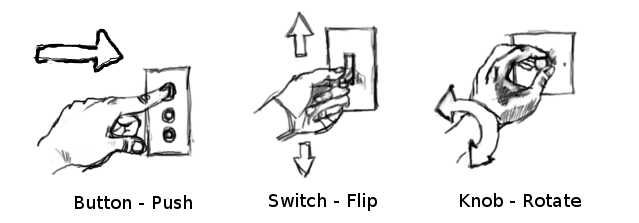
\includegraphics[scale=0.40]{fig-report/switches-only.png}
\caption{By their forms, buttons,switches or knobs often suggest their working.}
\end{figure}

Perceived affordance is not real affordance (\cite{affordancesMads}): design can rarely explain the complete working of complex objects. Perceived affordance shows primitive properties of its usage. This is why a bad design induces a difficult usage of the object, such as in Fig.~\ref{fig:lift-bad-design}.

\begin{figure}[h]
\centering
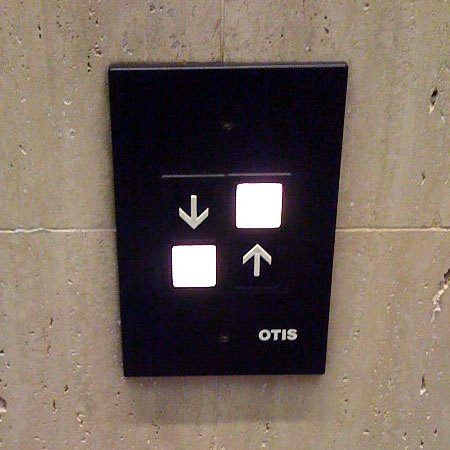
\includegraphics[scale=0.20]{fig-report/bad-switches.jpg}
\caption{What would you do in front of such a lift panel?}
\label{fig:lift-bad-design}
\end{figure}

    \subsubsection{Natural mapping}
\begin{defn}
Natural mapping is the idea of organizing controllers in the same arrangement as the objects on which they have an influence. It is one technique that can be used to achieve a good perceived affordance.
\end{defn}

A common example is the placement of the buttons that control the different stoves in a kitchen (see Fig.~\ref{fig:natural-mapping-1}~\&~\ref{fig:natural-mapping-2}, taken from \cite{stoveMapping}). It's obvious that the most left-top button will regulate the temperature of the most left-top stove.\\
 \begin{minipage}{\linewidth}
      \centering
      \begin{minipage}{0.45\linewidth}
          \begin{figure}[H]
          \centering
              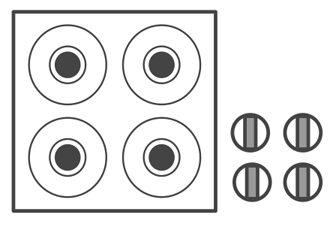
\includegraphics[scale=0.3]{fig-report/stove_natural.png}
              \caption{Scheme of a four stoves set with their corresponding knobs with natural mapping}
              \label{fig:natural-mapping-1}
          \end{figure}
      \end{minipage}
      \hspace{0.05\linewidth}
      \begin{minipage}{0.45\linewidth}
          \begin{figure}[H]
                    \centering
              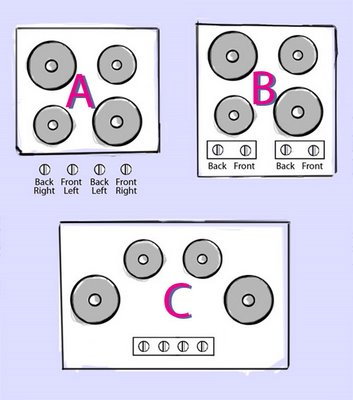
\includegraphics[scale=0.4]{fig-report/NormanBurners.jpg}
              \caption{Knobs arrangement without natural mapping, with varying success in perceived affordance.}
              \label{fig:natural-mapping-2}
          \end{figure}
      \end{minipage}
  \end{minipage}
  \bigskip

Unfortunately, this principle induces extra design cost and also depends on the point of view of the designer: even if it seems logical for certain arrangement such as stoves or the control of the electronic windows of the car, one can still doubt about the mapping of light switches(\textit{"Does the highest switch controls the front lights?"}).

    \subsubsection{Feedback}
\begin{defn}
\textit{\textbf{Feedback}}: sending information back to the user about his actions and their consequences.
\cite{Norman02}
\end{defn}

Feedback represents any action that could indicate to the user that its interaction with the item was taken into account. In certain cases, feedback can be done implicitly by the quality and the design of the object itself. For example, some buttons make a clicking sound when pressed. With modern technology however, feedback often requires additional functions like vibration or sound that corresponds to states of the device (see Fig.~\ref{fig:feedback}). These retro-actions have to provide the user with enough information to prevent a mistaken usage to cause frustration.

\begin{figure}[h]
\centering
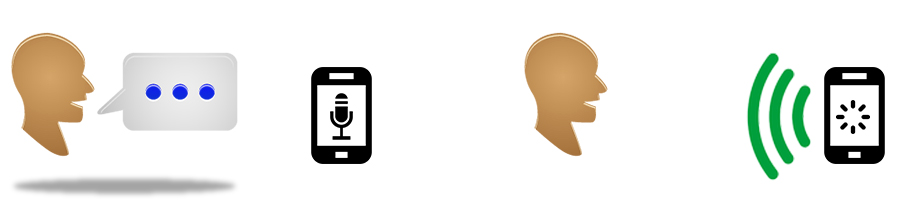
\includegraphics[scale=0.5]{fig-report/retro-action-speaking.jpg}
\caption{After the user gives a command, the device emits a sound to confirm that it is analysing the request}
\label{fig:feedback}
\end{figure}

    \subsubsection{Additional design principles}

While perceived affordance and constraints are the two main concept in object design, the author of \cite{Norman02} also presents the following concepts:

\begin{description}
    \item [Conceptual model:] Or ``how the user thinks it works''. The idea is to provide a precise information model about the correct usage or maintenance of the object. The design of such scheme is really important and should be extremely clear. Indeed, if it's not, the user may be frustrated when the object is not working. An example is given in Fig.~\ref{fig:concept-model}.

    \item [Make things visible] Certain of our modern items can be seen as real complex state machines due to the number of actions they can propose, causing the need for a display showing the current state and available actions. A good example is VoIP telephones allowing users to start a conference call with several other people, such as in Fig.~\ref{fig:make-things-visible}. Such telephones are equipped with a large display which can show different contacts numbers, propose features to start conference call or even to place a call on hold in order to answer to another call.
\end{description}

 \begin{minipage}{\linewidth}
      \centering
      \begin{minipage}{0.45\linewidth}
          \begin{figure}[H]
          \centering
              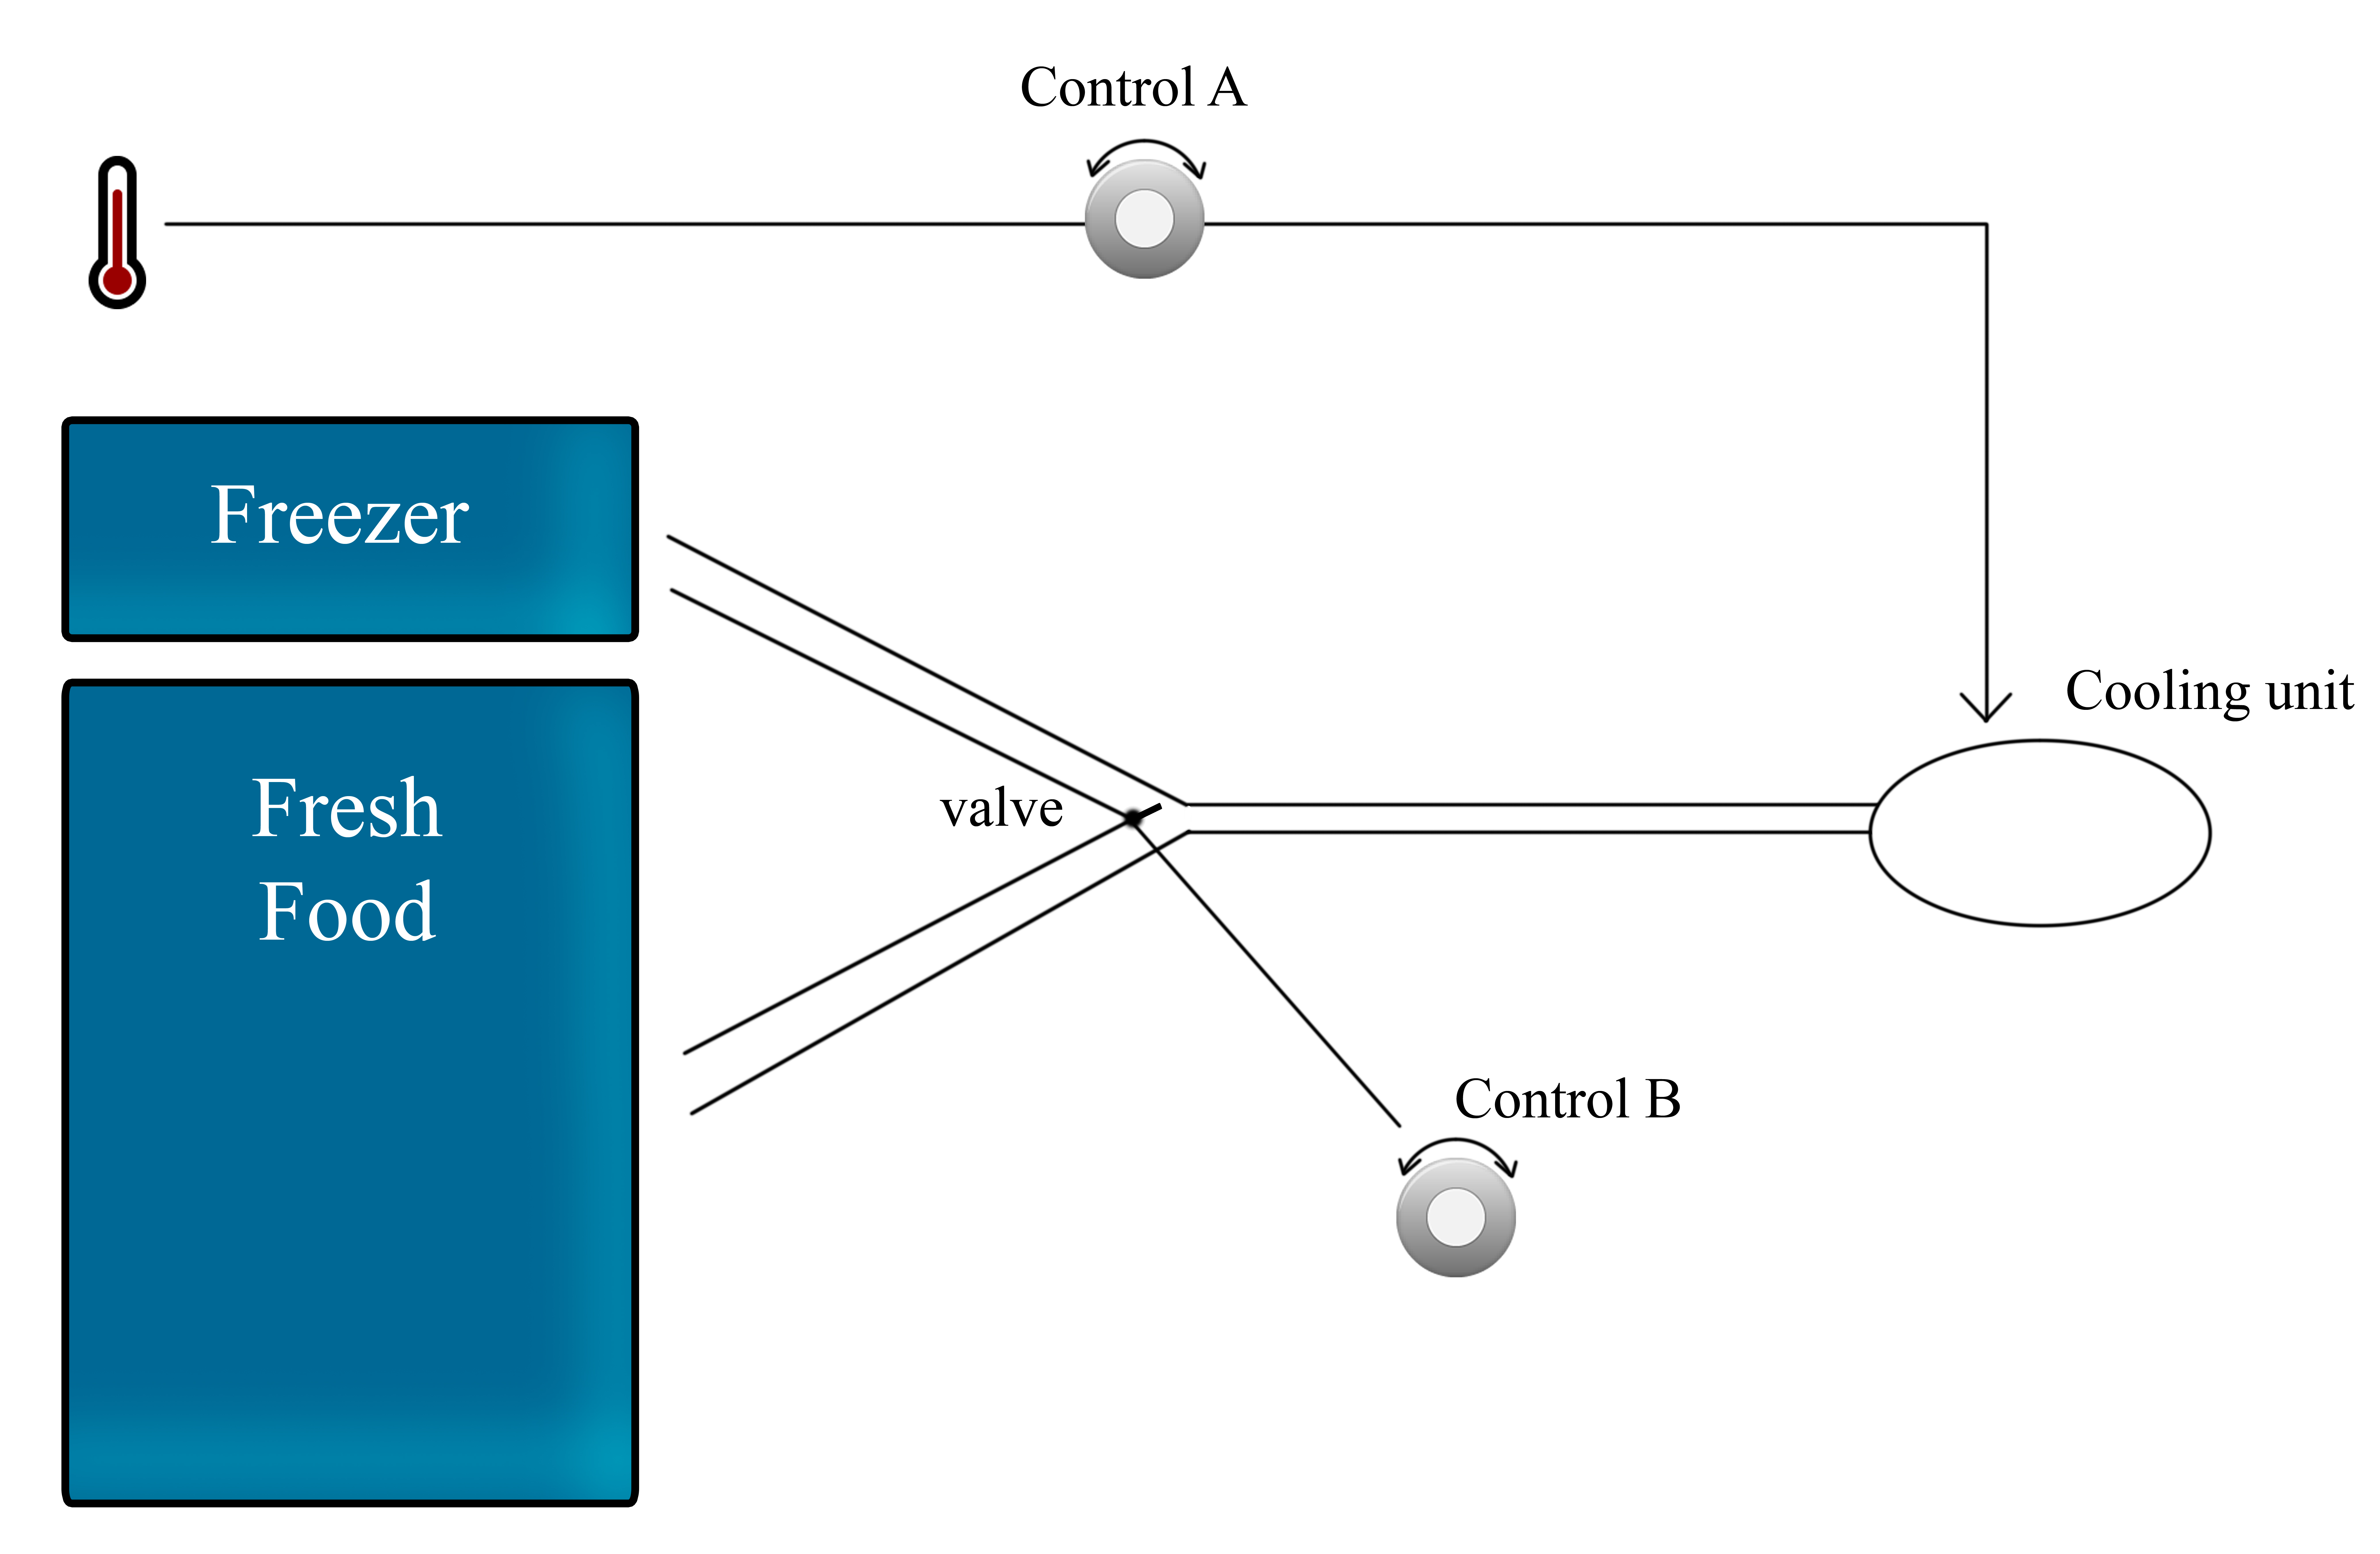
\includegraphics[scale=0.1]{fig-report/conceptual.jpg}
              \caption{Conceptual model of a freezer, inspired by a figure in \cite{Norman02}, the inner working may be more complex, but this is all the user need to understand}
              \label{fig:concept-model}
          \end{figure}
      \end{minipage}
      \hspace{0.05\linewidth}
      \begin{minipage}{0.45\linewidth}
          \begin{figure}[H]
                    \centering
               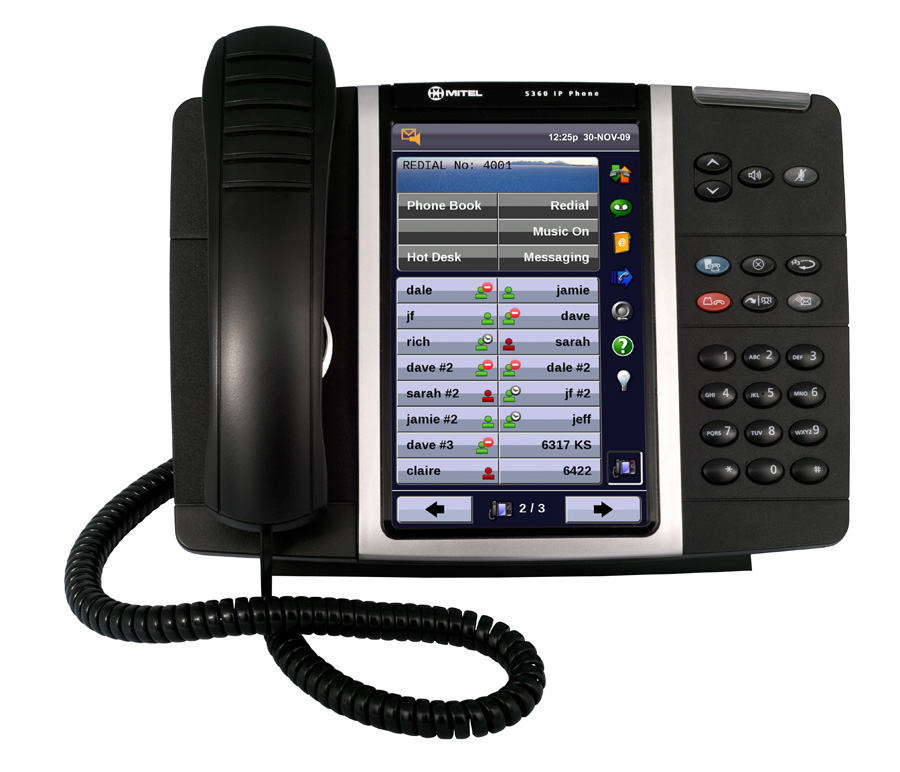
\includegraphics[scale=0.7]{fig-report/voip-phone.jpg}
              \caption{This complex VoIP phone uses a big display to explain its state and possible inputs to the user}
              \label{fig:make-things-visible}
          \end{figure}
      \end{minipage}
  \end{minipage}

    \subsection{Constraints}
    In addition to perceived affordance, usage of objects is also induced by different types of constraints. These constraints allow the user to immediately discard an incorrect interaction of the object.

        \subsubsection{Physical constraints}
        These constraints are the strongest because they considerably reduce the number of possible usages: they make incorrect usages clearly not physically possible, preventing the user to even try them. Such constraints do not or weakly depend on the knowledge of the user.\\

        $\underline{Example:}$\\
        Due to the design of the toolbox in Fig.~\ref{fig:phys-constr-toolbox}, it's completely impossible for the user to put, for example, his hammer into the slot reserved for a screwdriver.
        \begin{figure}[h]
        \centering
        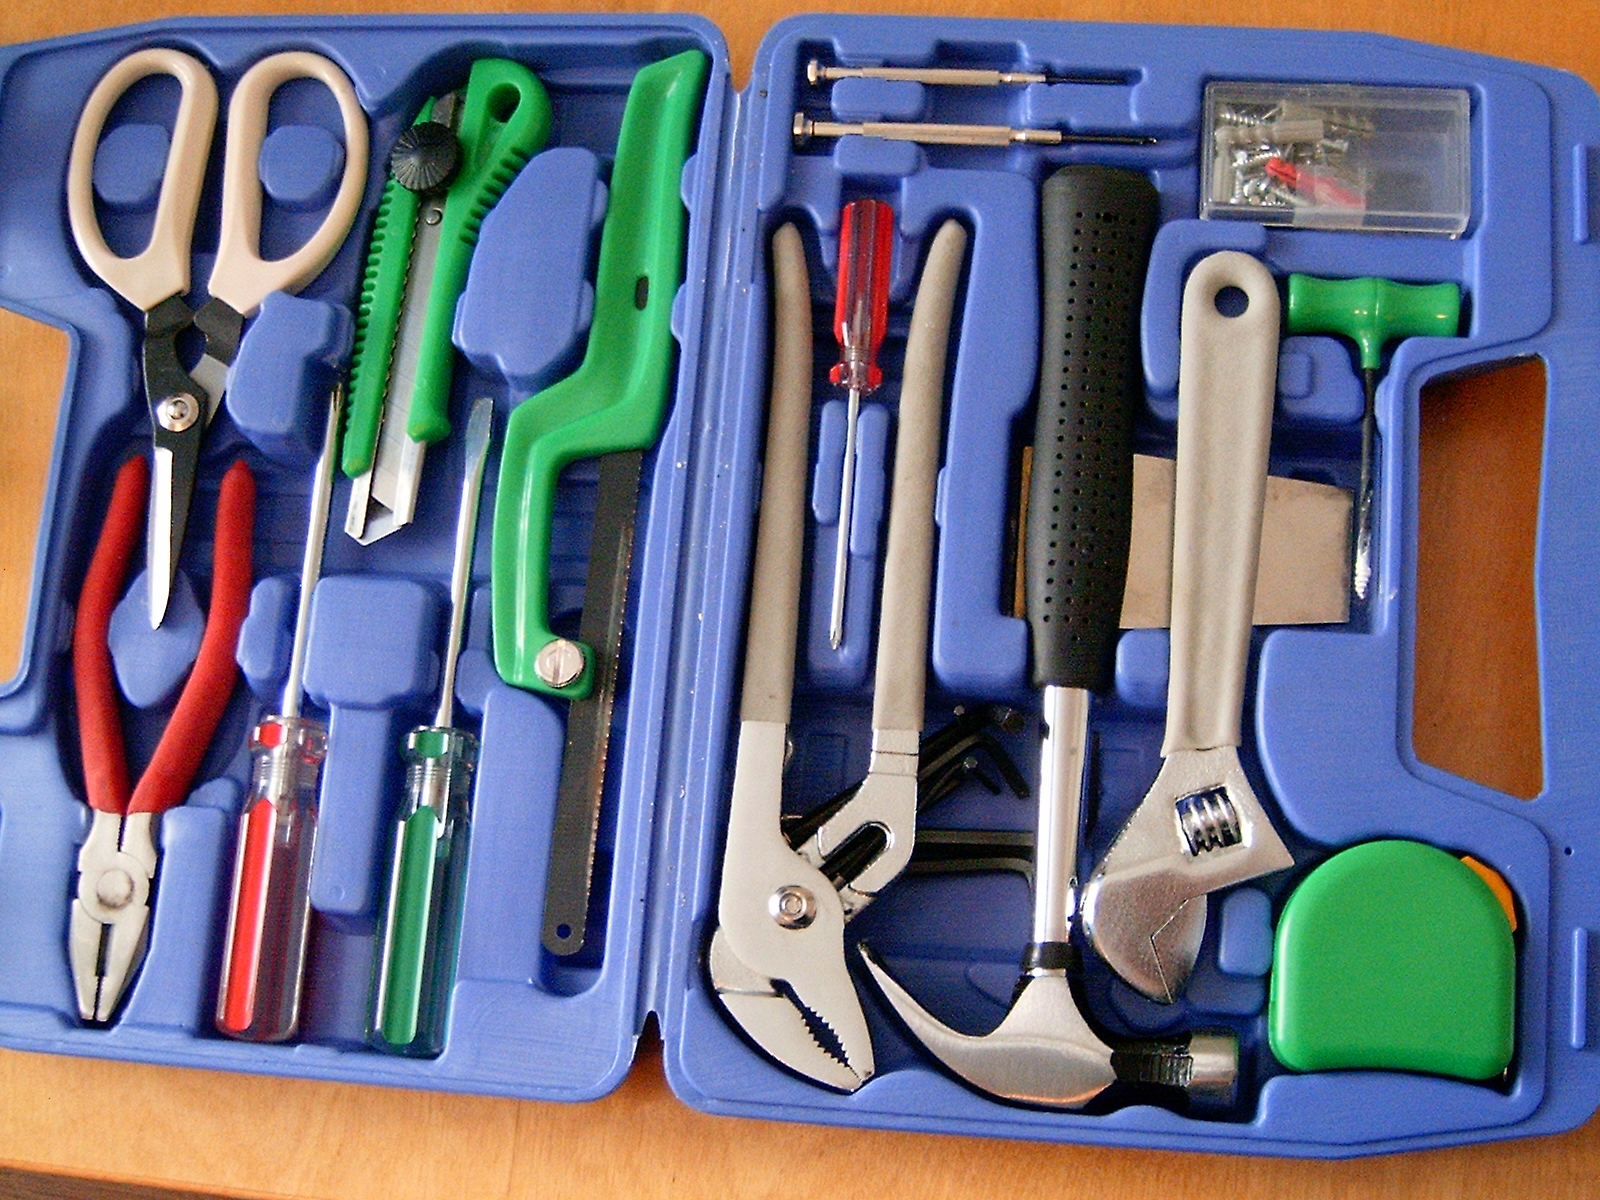
\includegraphics[scale=0.1]{fig-report/toolbox.jpg}
        \caption{A toolbox designed with physical constraints}
        \label{fig:phys-constr-toolbox}
        \end{figure}

        \subsubsection{Semantic constraints}
       In opposition to physical constraints, semantic constraints require a good knowledge of the situation in which the object should be used.\\

        $\underline{Example:}$\\
        Shoes design often supposes that the user knows how to make a correct knot. Users will discard alternatives because they have knowledge of the situation.

        \begin{figure}[h]
        \centering
        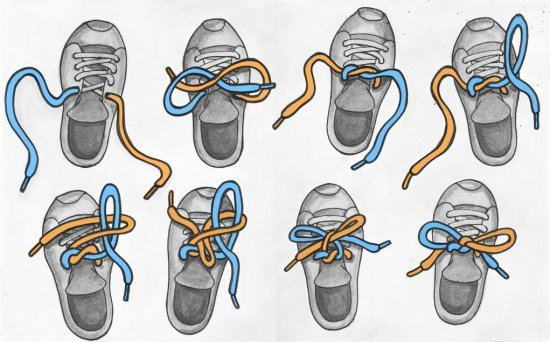
\includegraphics[scale=0.3]{fig-report/tie_your_shoes.jpg}
        \end{figure}

        \subsubsection{Cultural constraints}
        These constraints are the consequences of cultural conventions. These constraints can be considered arbitrary because in most of the cases, several possible alternatives could be applicable. Indeed such constraints do not affect the semantic or physical usage of the given object. Unfortunately, these constraints may change depending on the the geographical and temporal context. Furthermore these constraints are not applicable to new type of objects.\\

        \begin{figure}[h]
        \centering
        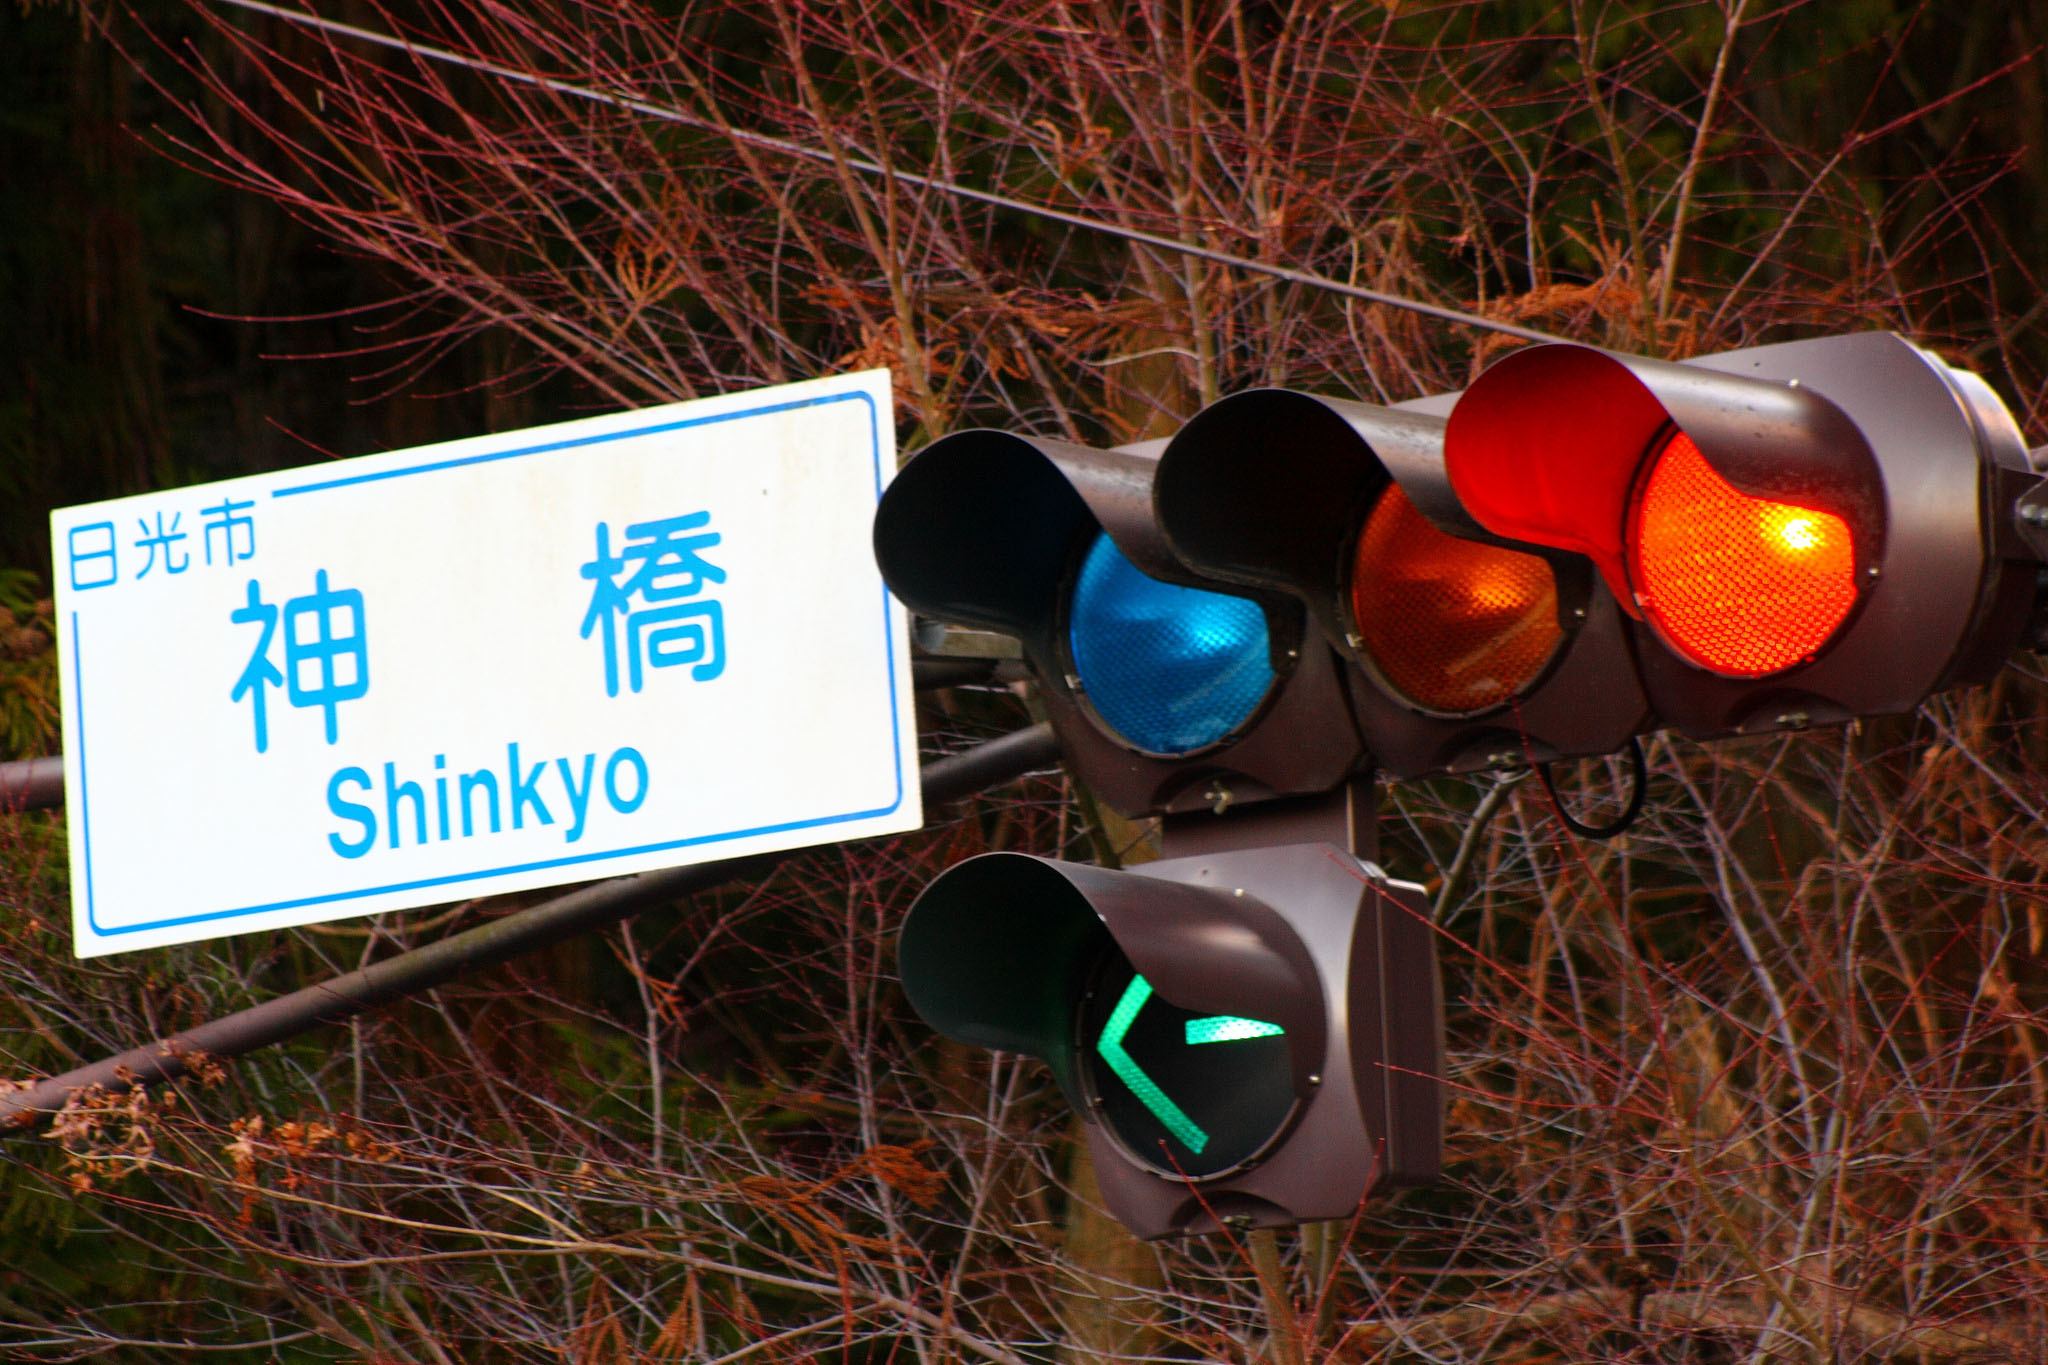
\includegraphics[scale=0.1]{fig-report/japan-traffic-light.jpg}
        \caption{Japanese traffic lights are designed with different cultural constraints}
        \label{fig:cultural-constr-traffic-light}
        \end{figure}

        $\underline{Example:}$\\
        An example is the disposition and color of traffic lights. In western countries, the green color means that you can pass, and traffic lights are positioned in a vertical column . In Japan however, traffic lights may be composed of blue, orange and red lights, and could be displayed as a horizontal row, such as in Fig.~\ref{fig:cultural-constr-traffic-light}.

        \subsubsection{Logical constraints}
        These constraints call to the good sense of the user, regardless of their physical or cultural knowledge. The correct usage should be the first and logical assumption of user through design choices. Such constraints are often linked to natural mapping.\\

        $\underline{Example:}$\\
        When using a frying pan where the handle is the only part which can be grabbed, the user will immediately understand its correct usage, as shown in Fig.~\ref{fig:log-constr-fryingpan}.

        \begin{figure}[h]
        \centering
        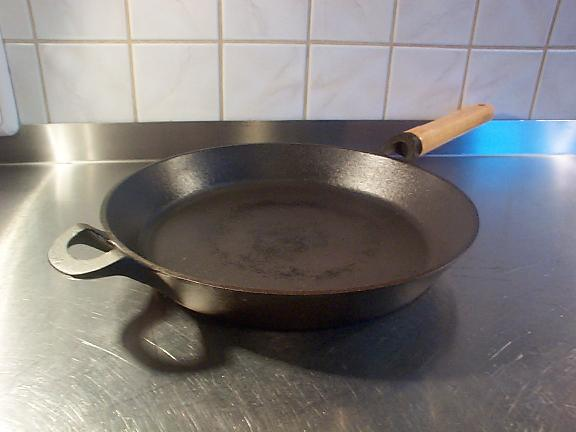
\includegraphics[width=0.45\textwidth]{fig-report/frying-pan-2handles.jpg}
        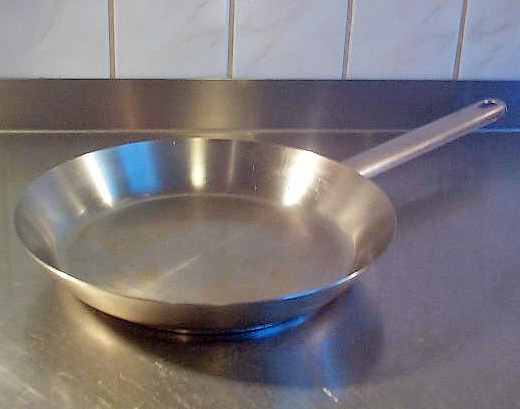
\includegraphics[width=0.43\textwidth]{fig-report/frying-pan-1handle.jpg}
        \caption{The frying pan on the right has less chance to be handled incorrectly, has there is only one handle to try}
        \label{fig:log-constr-fryingpan}
        \end{figure}

\newpage

\section{Evolution of computers interface}
\label{sct:history}

    \begin{figure}[h]
        \centering
        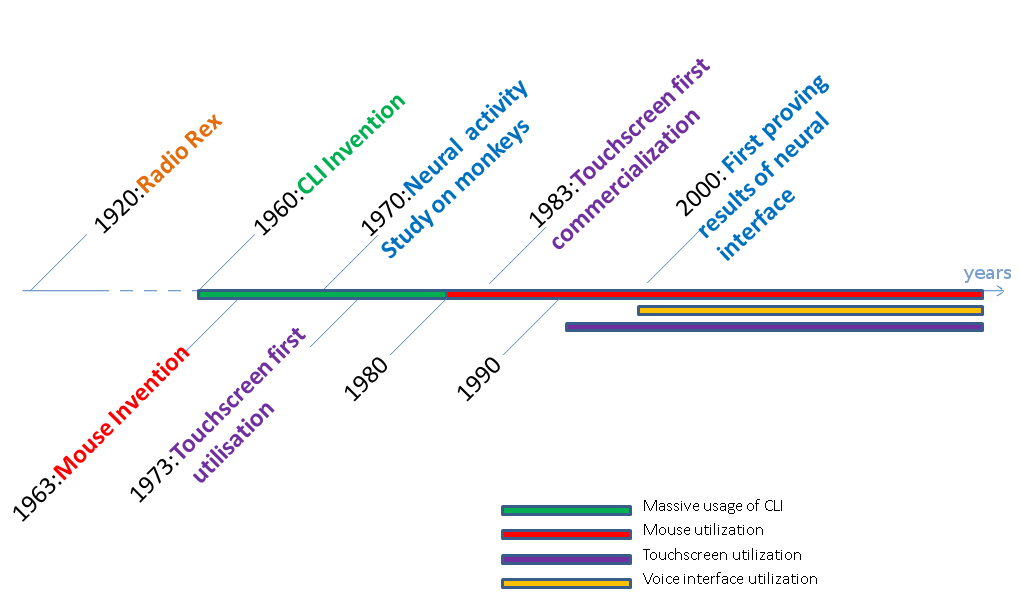
\includegraphics[width=0.75\textwidth]{fig-report/timeline-interface_2.png}
        \caption{Main events in the evolution of computer interfaces}
        \label{fig:timeline}
    \end{figure}

    As soon as computers became available to the public, the question of design came into play. While early designs were rough as computers were mainly aimed at professional use, the trend of personal computing brought a need for refined designs aimed at non-technical users. In this section, we present different types of computer interfaces for personal computing devices and explain them in terms of design principles.

    \subsection{Command line interpreter (CLI)}

    \begin{figure}[h]
        \centering
        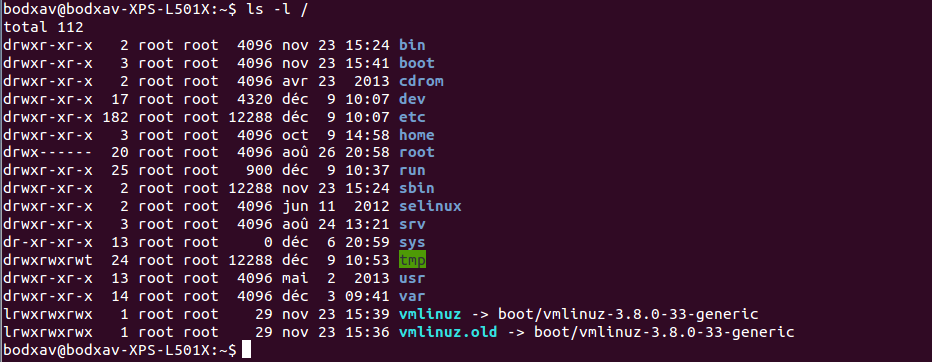
\includegraphics[width=0.95\textwidth]{fig-report/terminal.png}
        \caption{A typical CLI showing the content of a directory. Color is used for highlighting certain informations}
        \label{fig:cli}
    \end{figure}

    The first attempt at an usable design for computing devices was the Command-Line Interface (CLI) (Fig.~\ref{fig:cli}). The user can interact with the device using a keyboard by typing commands to launch programs, then the output of the program is displayed on the screen. While typing, the current command is displayed next to a cursor to provide feedback to the user. The buttons of the keyboard are labeled and follow a pattern standardized by countries, which is a case of natural mapping and cultural constraints.\\

    Command-line interfaces were introduced in the 1960s and remained a de-facto standard until the introduction of graphical interfaces. Later iterations were improved by features as auto-completion (which improved the perceived affordance of possible commands) and colors (which helped the user to build a conceptual model). Note that while CLI are not used as a main interface in personal computers anymore, advanced users still use them in certain cases due to their efficiency.

    \subsection{Graphical interface and computer mouse}

    Invented in 1963 and made famous in 1968 during the ``Mother of All Demos''\cite{engelbart1968research}, the computer mouse (Fig.~\ref{fig:mouse}) coupled with an OS using a graphical interface (Fig.~\ref{fig:gui}) allow the user to interact with the space of the screen. Graphical interfaces allowed designers to use powerful visual metaphors to construct an intuitive conceptual model (i.e. start button, trashbin, desktop, etc), as well as providing visual feedback to the user (movement of the mouse cursor, highlighting of selected items, animation when minimizing program).\\

    Graphical interfaces and their intuitive conceptual model helped the broad adoption of personal computers. They are still the main interfaces used today, even if some operating systems are now pushing for a shift to touch interfaces. The latest iterations concentrate on higher-resolution icons and more complex animations.
 \begin{figure}[H]
    \centering
    \
    \end{figure}
    \begin{figure}
   \begin{minipage}[c]{.46\linewidth}
      \centering
      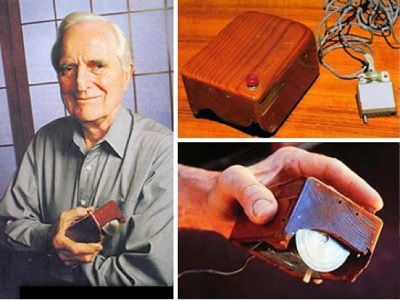
\includegraphics[scale=0.8]{fig-report/first-mouse.jpg}
    \caption{Douglas Engelbart and the first computer mouse that he invented in 1963\cite{douglas}}
      \label{fig:mouse}
   \end{minipage} \hfill
   \begin{minipage}[c]{.46\linewidth}
   \centering
         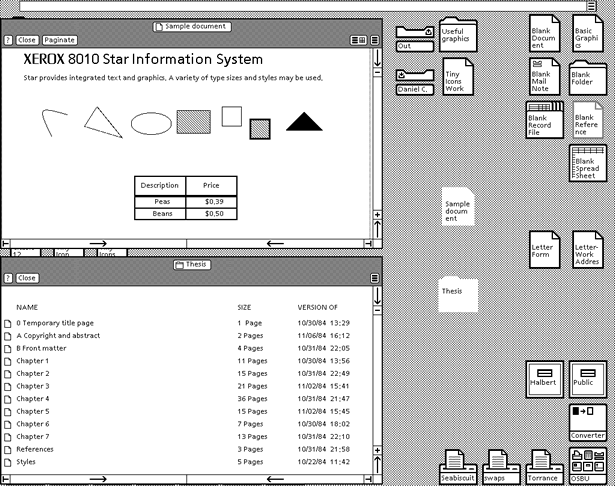
\includegraphics[scale=0.4]{fig-report/xerorx-8010-star.png}
         \caption{Xerox 8010 Star interface is the first GUI ever commercialized (Around 1981)\cite{xerox8010}}
         \label{fig:gui}

   \end{minipage}
\end{figure}

    \subsection{Touch interface}


    Introduced in 1973, the touchscreen seems to be the logical evolution of the computer mouse, as it allows 
   
    the user to interact directly with the screen rather than using peripheral devices such as the mouse and the keyboard. Touch interfaces may use virtual and familiar devices such as buttons and switches whose affordance will be instantly recognized by the user, and actions such as moving a file or resizing an image can also be accomplished by intuitive movements such as dragging a finger across the screen or using to fingers to pinch.\\
\begin{figure}[!h]
\centering
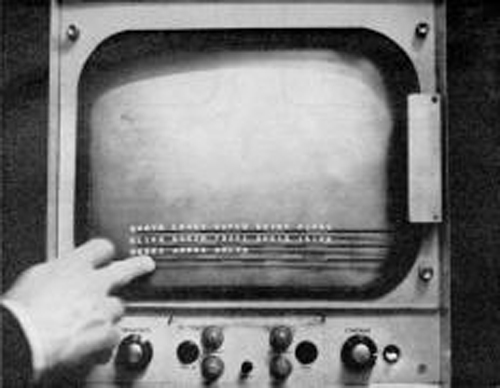
\includegraphics[scale=2]{fig-report/first-touchscreen.jpg}
\caption{First invented touchscreen by E.A. Johnson in 1965 at the Royal Radar Establishment in Malvern, United Kingdom\cite{first-touchscreen}}
\end{figure}
    While touchscreens seem to be a straight upgrade in terms of conceptual model, they lack the precision and haptic feedback given by the mouse and keyboard. While this problem is partially solved by advances in technologies and vibrators embedded in the device, touch interfaces are not used in the majority of personal computers nowadays, especially in professional environments. However, the technology is now widely used in smartphones and in the new market of electronic tablets.

    \subsection{Voice interface}

    With early appearances as soon as in the 1920s, voice interfaces is an old idea whose usability is highly dependent on advances in the fields of speech recognition and semantical analysis. While the latest commercial voice interfaces allow to recognize many languages with a low rate of errors, current interfaces only allow users to input simple commands in a limited set of languages. They are rarely used by most users (as found by \cite{SiriNotUsed} which studied Apple's Siri), so we chose not to concentrate on it in this report.

    \subsection{Neural interface}
    With the latest development in neuroscience, designers are able to limit the interface to a single chip in the brain of the user. Such technology is mainly dedicated to disabled people who cannot use the previously described interfaces. For example, Brown University researchers succeeded in helping a paralyzed woman to move a robotic arm with a wireless chip implemented in her brain \cite{brownRobotic}. Transmitting information directly from the user's brain to a machine could in the future become more affordable and a new standard in term of interface design.

    \begin{figure}[!h]
    \centering
    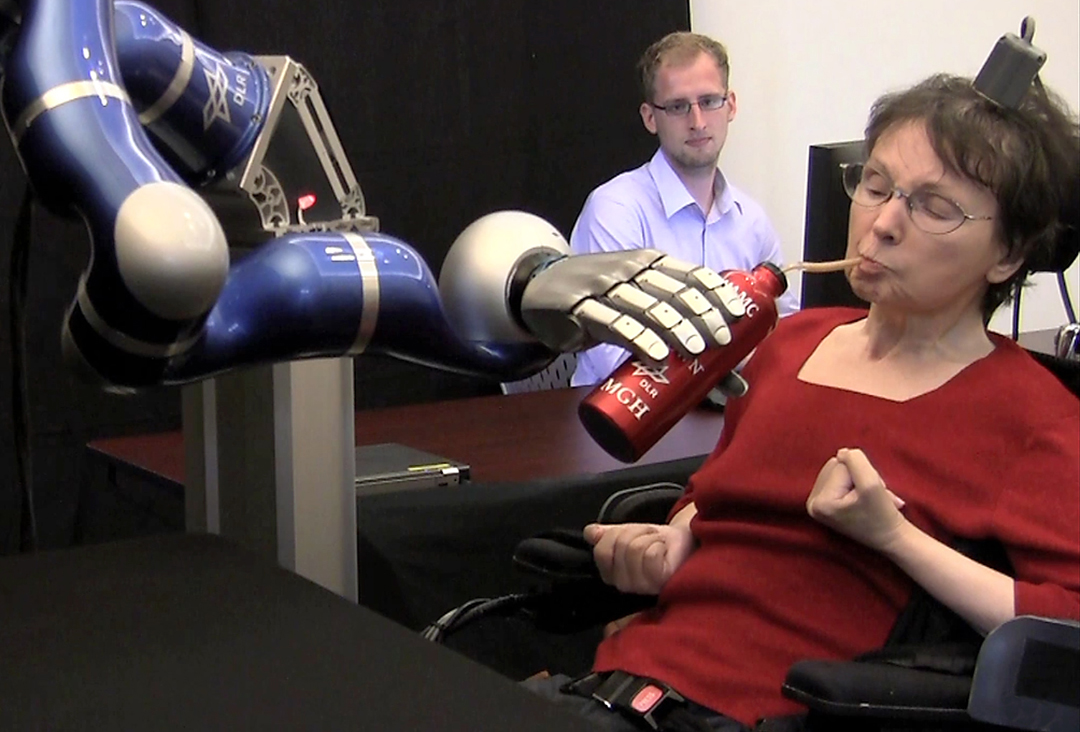
\includegraphics[scale=0.15]{fig-report/robotic-arm-brain.jpg}
    \caption{A 58-year-old woman, paralyzed by a stroke for almost 15 years, uses her thoughts to control a robotic arm, grasp a bottle of coffee, serve herself a drink, and return the bottle to the table\cite{brownEdu}.}
    \end{figure}

    \subsection{Current trends in touch interface}

    Early design of touchscreen devices were often derived from classical mouse-based design, with the screen touches interpreted as mouse clicks. These devices remained a niche market until the introduction of devices designed from the ground up for touch-based devices. We now present two design paradigms which are used nowadays for these type of devices.

        \subsubsection{Skeuomorphism}
        \begin{defn}
        \textit{Skeuomorph:} An object or feature which imitates the design of a similar artefact made from another material. From the greek words $\sigma \kappa \varepsilon \upsilon {\rm o} \zeta$ (tool) and $\mu {\rm o} \rho \varphi \eta$ (shape).
        \end{defn}

        This design paradigm was first introduced in 2007 with Apple's iOS operating system for their iPhone and iPad devices, both highly successful and followed by other devices with a similar design. Skeuomorphic applications try to mimic an existing object in order to feel familiar to the user.\\


        For example, a skeuomorph dialer application may display a picture of an analog wheel-shaped dialer and asks
 
        the user to turn the virtual wheel in a movement familiar to him. While the user is inputting a number, the application may play the sounds of the wheel turning and a bell ringing. This type of application has very clear affordance, an intuitive conceptual model and provides efficient feedback, as long as the user is familiar with the mimicked tool.\\

        Skeuomorphic applications are often characterized by realistic textures, glossy elements and gradient backgrounds, resulting in a three-dimensional feel.

        \subsubsection{Flat design}
        \begin{defn}
        \textit{Flat design} \cite{whatIsFlat}: minimalistic design approach that emphasizes usability. It features clean, open, crisp edges, bright colours and two-dimensional/flat illustrations.
        \end{defn}

        While skeuomorphic designs helped the broad adoption and usage of touch-based devices thanks to their familiar conceptual model, they also add many superfluous details which can distract the user from the relevant usage of the application. Their complex design can cause a higher battery usage and eye fatigue to the user, as well as limiting the usability of the application to the one of the object it tries to mimic (for example, a truly skeuomorphic dialer cannot autocomplete phone numbers based on the user's contact list).\\

        Hence the recent rise of the Flat design, in which all superfluous elements are removed. These designs tend to be minimalist and to have a two-dimensional iconic feel. An early example is the controversial \textit{Metro} interface for Windows 8, and later the iOS7 update which signified a paradigm shift in Apple's design. Fig.~\ref{fig:skeuoflatCompare} shows an example of both design.

 \begin{figure}[H]
    \centering
    \
    \end{figure}
    \begin{figure}
   \begin{minipage}[c]{.46\linewidth}
      \centering
      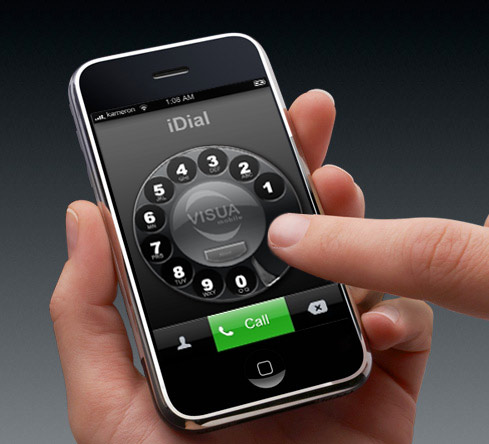
\includegraphics[scale=0.4]{fig-report/idial.jpg}

   \end{minipage} \hfill
   \begin{minipage}[c]{.46\linewidth}
   \centering
         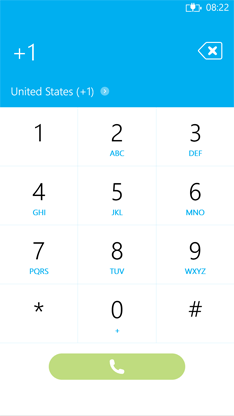
\includegraphics[scale=0.5	]{fig-report/dial-flat.png}
   \end{minipage}
   \caption{Skeuomorphic and Flat design of a dialer application}
   \label{fig:skeuoflatCompare}
\end{figure}
\section{Experiments}
\label{sct:experiment}

    \subsection{Definition of the experiment}

    To compare skeuomorph and Flat design, we presented our subjects with two different calculator applications on iPad. The first one, m38+, had a familiar skeuomorph design and the other, Soulver\footnote{Developped by Acqualia: \url{http://www.acqualia.com/soulver/}}, had an original but intuitive design, based on Flat principles. After a quick demonstration of both apps, the subject was asked to answer simple questions using both applications. The quiz is available as an appendix.\\
 \begin{figure}[H]
    \centering
    \
    \end{figure}
    \begin{figure}
   \begin{minipage}[c]{.46\linewidth}
      \centering
      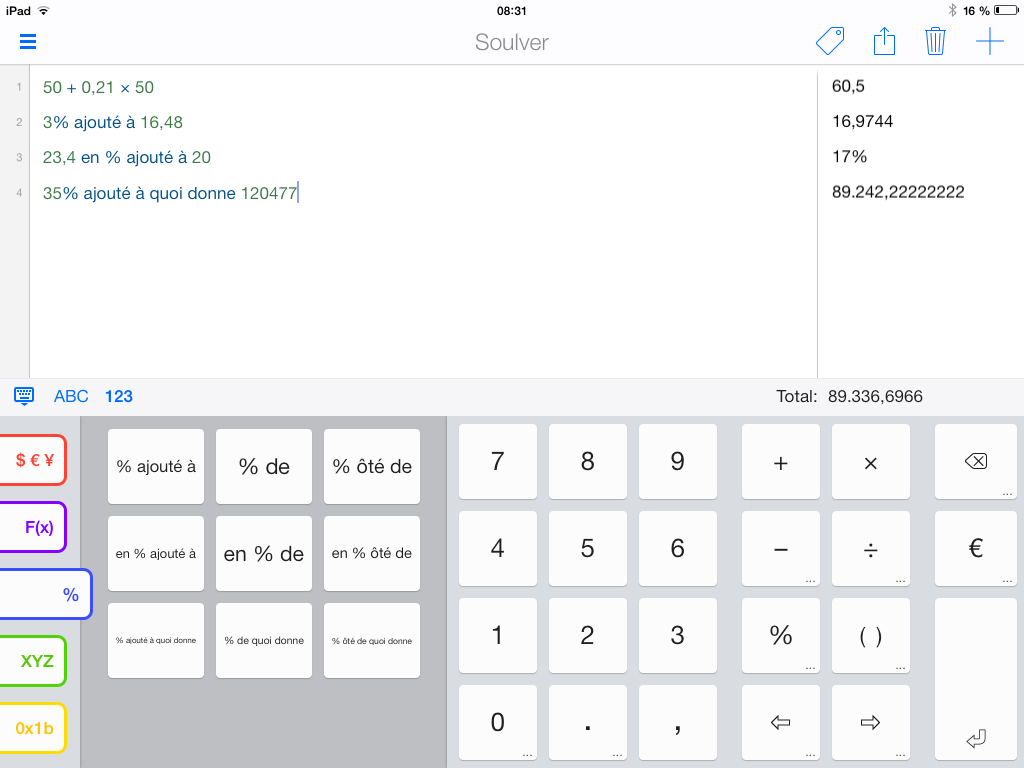
\includegraphics[scale=0.2]{fig-report/soulveur-screen.png}
         \caption{Flat design of the Soulver app}
   \end{minipage} \hfill
   \begin{minipage}[c]{.46\linewidth}
   \centering
         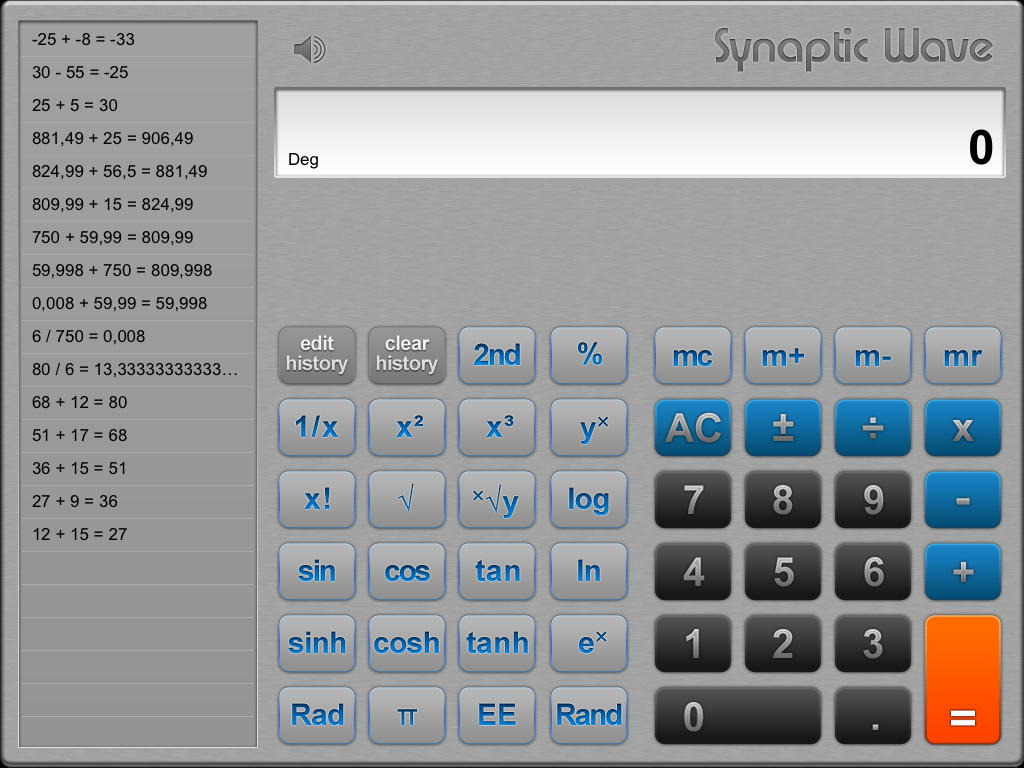
\includegraphics[scale=0.2]{fig-report/m38-screen.png}
         \caption{Skeuomorph design of the M38+ calculator}
   \end{minipage}

\end{figure}


    \subsection{Results analysis}

    \subsubsection{First exercise: travel bill}

    Subjects were asked to calculate expenses made during a trip, based on various receipts. Most chose the skeuomorph calculator. We suppose that due to the apparent simplicity of the operations, they assume the familiar calculator will be sufficient. In general, the subjects arrived at the correct amount.\\

    When we asked them to give us only the money spent on taxi fares, they could not answer because the computation steps were not labeled. Note that this is not possible with a real calculator either. When the flat calculator was used, the subjects tend to use as many features as possible (labels, dedicated functions). As a result, the users were able to tell us about the details of the bill.\\

    Some subjects had a problem with the skeuomorph calculator as it was not working as the ones  they daily use (especially the syntax of the percent function). In that case, the skeuomorph design loses its usability gain and even harms the conceptual model of the user.\\

    \subsubsection{Second exercise: tax computation}

    In the second part of the experiment, we forced the subjects to choose the other calculator (Most of the time, \textit{Soulver}).\\

    Most of the subjects were lost due to uncommon interface. Indeed, the numeric pad is not highlighted and Soulver proposes many functions (such as percent computation or simple equation solving). Instead of using dedicated functions, they tried to use their mathematical knowledge to solve the equations. As a consequence, results (but also computation time) were not as good as in the first exercise.\\

    Once we showed them the additional functions in details, users appeared to be pleasantly surprised that the application integrates such features: Most of them explained us that they didn't see it because it's not emphasized and suggested that developers should use different button designs (color, shape, text color, etc). A well-received feature of the flat calculator is the fact that it integrates a labeled history in which users can add textual information, making the sub-resolution problems easier.\\

    In general, users couldn't use the full potential of the flat calculator due to the lack of information. At first sight, and due to a limited design, users appeared lost and limited their actions to the simple arithmetic instead of exploiting the dedicated functions to compute percentage or solve basic equations. Several users admitted that they wanted to use the flat calculator for everyday operations (shopping list, bills, etc), but only after a small training session because to counterbalance their lack of mathematical knowledge.\\

    \subsubsection{Third question: Flat design in practice}
    In conclusion to our experiment, we asked our subjects what they thought of either the new design of iOS 7 proposed by Apple or the interface of Microsoft's Windows 8, whichever was the most familiar to the subject.\\

    Subjects estimated that the new flat design is more beautiful and abstract without much loss in terms of usability, even if older users admitted that the flat design required a short adaptation:
  	(In french) \textit{Colette} - \textit{"Lors de la mise à jour, j'ai été surprise et un peu perdue parce que toutes les icones avaient changées. Après deux ou trois jours d'utilisation, je me suis adaptée. Si on devait revenir au précédent design, ce serait une perte de temps étant donné que je devrais m'y ré-adapater."}

    \subsection{Comparison with previous experiments}

    During our research, we encountered a lack of objective and reputable studies on the subject, making it difficult to get a big picture. The three studies we present here are:
    \begin{itemize}
        \item A post on a design blog which surveyed icon preference amongst its reader
        \item A report by Microsoft over user preferences between Windows 7 and Windows 8
        \item A study from a Japanese university which analyzed different types of icons and classified them using design factors.
    \end{itemize}

    \subsubsection{Flat VS skeuomorphism}

    The first survey \cite{flatVSskeuomorphisme} asked users to choose their favorite design amongst a set of icons from Android, iOS6, iOS7 and Windows Phone. The results are shown in Fig.~\ref{fig:flat-vs-skeu-result}\\

    \begin{figure}[h]
    \centering
    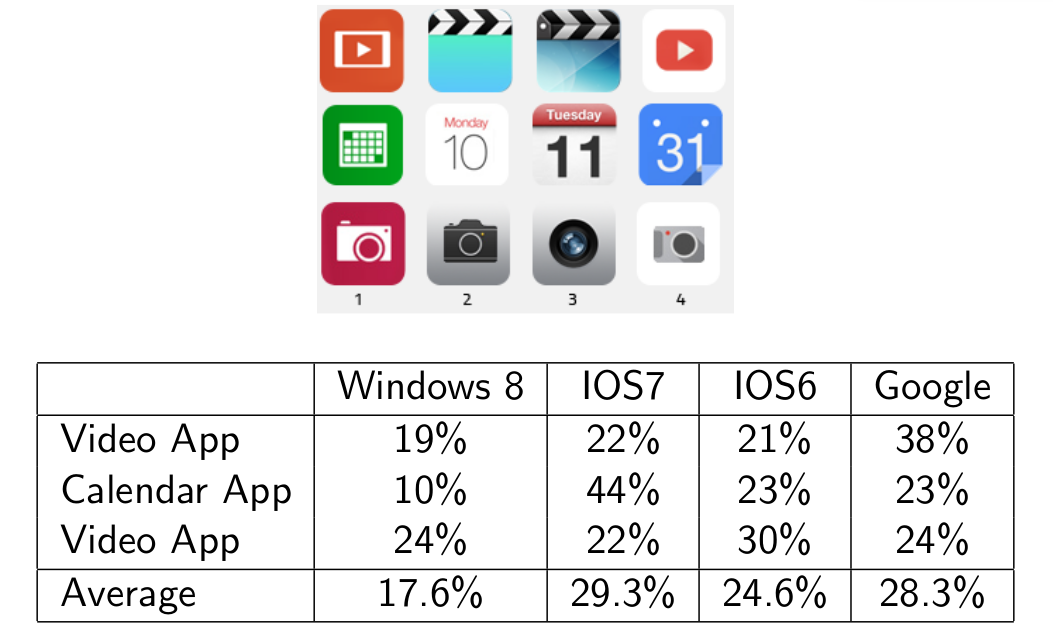
\includegraphics[scale=0.3]{fig-report/flatVSskeuomorphism.png}
    \caption{Preference of 2000 users as found in \cite{flatVSskeuomorphisme}}
    \label{fig:flat-vs-skeu-result}
    \end{figure}

    Considering that only iOS6 is based on skeuomorph principles, we see that more than 70\% of the participant voted for flat icons in each case. Note that results are influenced by the majority of flat icons amongst the choices.\\

    An interesting point is the calendar icon of Windows Phone, which obtains the lowest number of votes. This could be explained by the fact that its design is very different from the three other calendar icons and does not immediately evoke a calendar.\\

    %The main problem with this study is that there is no skeuomorph icons for google and windows phone. The majority of the icons being flat influence the results so that this is hard to belief. Another interesting thing is that windows 8 got a really low score for his calendar application. The three other possibilities looks similar and got an higher scores, leading to the conclusion that people really do not like this icon.

    We conclude that even if the study is not completely objective, users appear to respond well to flat design principles and prefer it to skeuomorphic designs in certain circumstances.

    \subsubsection{Windows 8 survey, half prefer windows 7}

    This survey\cite{windows8Survey} is made by Microsoft using Windows users as subjects, and thus should be taken with care. That being said, the information revealed by the survey is quite interesting. The Metro UI (flat user interface) is ranked at the 9th position of the most liked features with 22\% of the people liking it. However, the presence of both Metro and classical desktop interface is disliked by 18\% of the people, ranking it at the fifth place of the weaknesses to be improved.\\

    We can observe that on average, voters have chosen twice as much liked features as weaknesses. Other surveys show that two Windows users out of three still uses Windows 7, a preference that could be caused by the price (35\% of the survey seeing this as one of the weaknesses) or other factors than the new UI.\\

    \begin{figure}[!h]
     \centering
     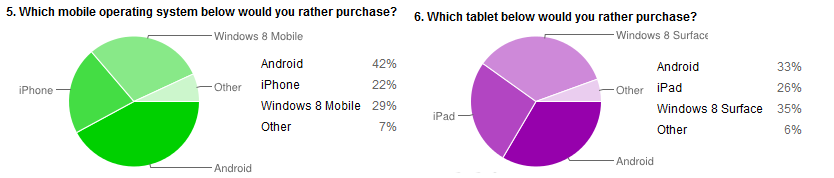
\includegraphics[scale=0.55]{fig-report/tablet.png}
     \caption{Polls results about mobile devices operating systems preferences, from \cite{windows8Survey}}
     \label{fig:windowsSurvey}
     \end{figure}

    Further results (presented in Fig.~\ref{fig:windowsSurvey}) shows operating system preferences. Note that the results are from September 2012, a year before the introduction of iOS7. Globally, Android dominates the market with a third of all mobile devices (phones and tablets). Both iOS6 and Windows phone have a quarter of the market in term of phones. One can notice that windows 8 surface leads the tablet market with 35\%.\\

    This means that while Android and IOS globally get the same part of the tablet market, Windows seems to be preferred on bigger touchscreen devices. This may be because its User Interface is designed for touchscreen computers and tablets. Knowing that Microsoft tried to offer an unified experience, we can conclude that several features are not well-designed for all devices.

    \subsubsection{A preliminary study on aesthetic of apps icon design}

    This study \cite{jpAnalitics} was made by a Japanese university with the collaboration of two members of the Department of Industrial Design National Cheng Kung University in Taiwan. It analyzed different aspectss of icons aesthetic, the links between them and their interactions with users. It also defined a frontier between skeuormophism and flat design. Results were obtained using evaluation grid results, quantification theory and regression (Fig.~\ref{fig:jppage8}) to identify potential relationships between components of the icons. They also introduced the kansei interface concept that includes emotional principles in the UI.\\

    The kansei interface is a principle based on usability, but adds a positive emotion factor with what they call interactive motivation. This is motivated by global application stores proposing multiple applications doing the same things. The developer goal is to attract the user towards their application by designing an attractive icon. It should create emotion to get interest, motivation to look further, and usability to understand the purpose.\\

    The experiment was separated in three parts:
    \begin{enumerate}
    \item Analysis of the aesthetic factor of a set of icons by designers
    \item Definition of height groups in order to define category of icons (Fig~\ref{fig:jpfig5})
    \item Polls in order to measure their feelings about selected icons (Fig~\ref{fig:jppage8})
    \end{enumerate}

     The third step consisted of a questionnaire asking users which type of icons they found attractive. The results (Fig~\ref{fig:jpfig6}) show that the more abstract an icon becomes, the less attractive it is. We can also observe that concrete icons have more success than abstract (flat) ones.

    \begin{figure}[H]
      \centering{
        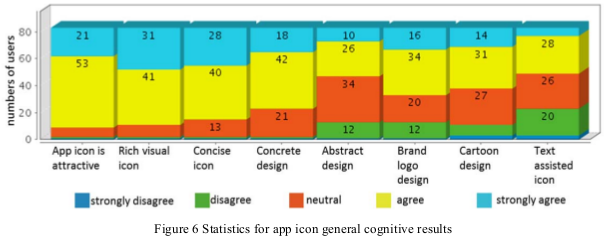
\includegraphics[scale=0.7]{fig-report/jpfig6.png}
      }
      \caption{Preferences of users amongst different icons, from \cite{jpAnalitics}}
      \label{fig:jpfig6}
    \end{figure}

    The following results are from another questionnaire asking users their preference amongst flat and skeuomoprh icons. Those results were used to build a correlation between previously analyzed factors and properties of the icon such as ``cute'', ``vigorous'', ``intuitive'' or ``fun''. For example, ``vigorous'' icons were those with a 3D effect, colors, dynamic elements and novelty. The full table is presented in the appendices (Fig.~\ref{fig:jppage8}). The aim of this was to define the axis of the map as concrete-abstract and detailed-terse(Fig.~\ref{fig:jpfig7}).\\

    Based on the map, another set of subjects was asked to compare concrete and abstract (or skeuomorph and flat design) icons. The results (Fig.~\ref{fig:jppage10}) show that most people prefer concrete style icons.

    \begin{figure}[H]
      \centering{
        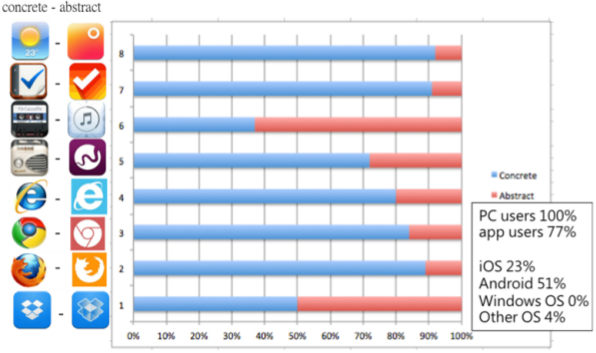
\includegraphics[scale=0.5]{fig-report/jppage10.png}
      }
      \caption{User preferences amongst abstract or concrete icons, from \cite{jpAnalitics}}
      \label{fig:jppage10}
    \end{figure}

\section{Conclusion}

In this document, we presented some of the ideas and challenges for the design of touch-screen based applications. In particular, we compared the two visual languages used in most tablet operating systems: Flat and Skeuomorph. Note that there are of course other factors to take into account when designing an application such as spatial layouts, color palette, screens arrangement, etc.\\

Skeuomorph designs were the norm when touch-based devices were first introduced to the public and have greatly helped their wide adoption. However, it now seems that both designers and users have grown tired of the inherent limitations of such designs. This leads to the current shift to more minimalist designs with sharp edges and bright colors, or Flat design.\\

While skeuomorphism worked well for non-technical people thanks to their immediate conceptual model, the shift to Flat forces application creators to concentrate even more on the design of their application, as it has to be intuitive. This was very clear in our experiment, where subjects instinctively chose the skeuomorph application over the Flat one, which offered more features but seemed complex to use. When using the flat application, our subjects often missed some of the more advanced features and seemed confused when asked to use them, highlighting a weak conceptual model.\\

We find similar results in other studies: flat-design is not sufficient to provide complete usability and can be even be worse than skeuomorphism in some cases. However, people are tired of skeuormophic design and tends to respond positively to flat,design. In our opinion, application developers should follow the current Flat design trend without forgetting the needs of a intuitive conceptual model, which is harder to achieve with such designs.
\newpage
\appendix

\section{Appendix - Figures of ``A preliminary study on aesthetic of apps icon design''}
Here are some relevant figures presented in \cite{jpAnalitics}.
  \begin{figure}[H]
    \centering{
      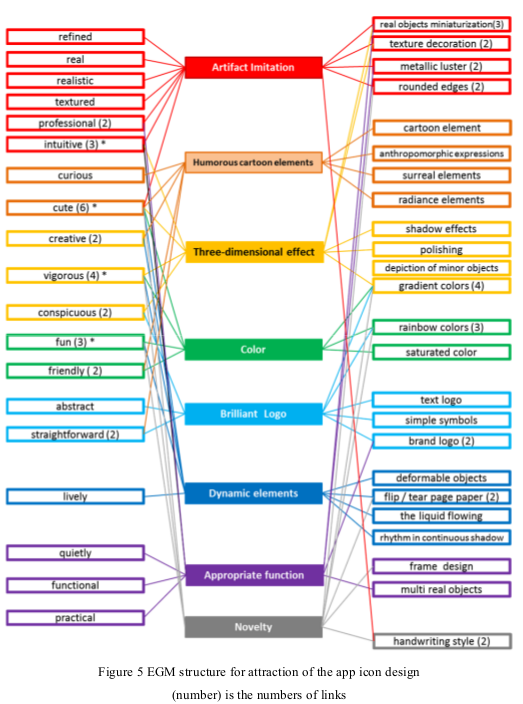
\includegraphics[scale=0.7]{fig-report/jpfig5.png}
    }
    \caption{Figure 5 of the study}\label{fig:jpfig5}
  \end{figure}

  \begin{figure}[H]
    \centering{
      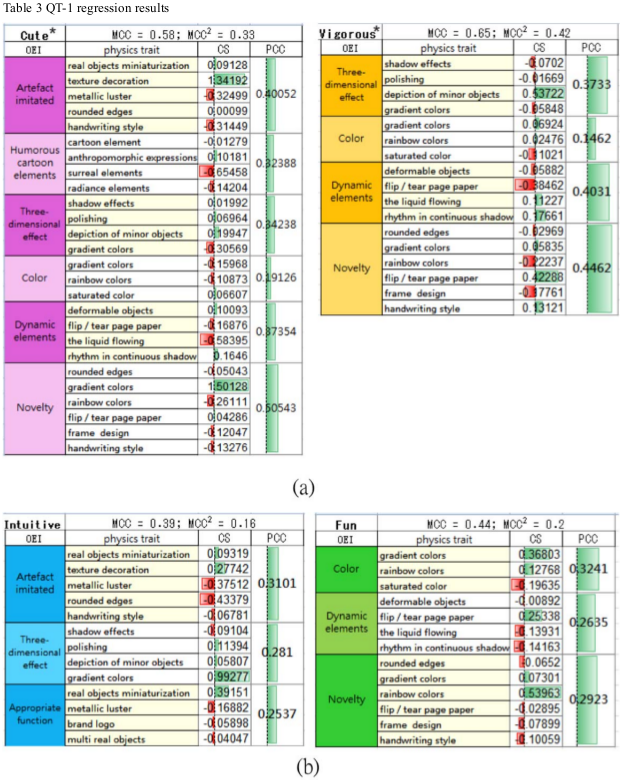
\includegraphics[scale=0.7]{fig-report/jppage8.png}
    }
    \caption{page 8 of the study}\label{fig:jppage8}
  \end{figure}
  \begin{figure}[H]
    \centering{
      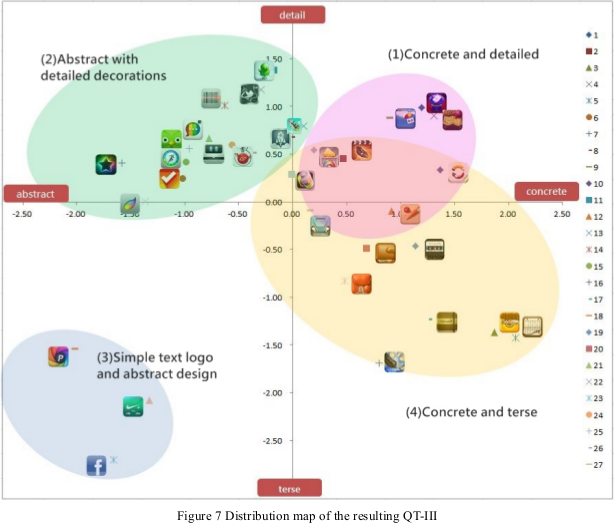
\includegraphics[scale=0.7]{fig-report/jpfig7.png}
    }
    \caption{Figure 7 of the study}\label{fig:jpfig7}
  \end{figure}

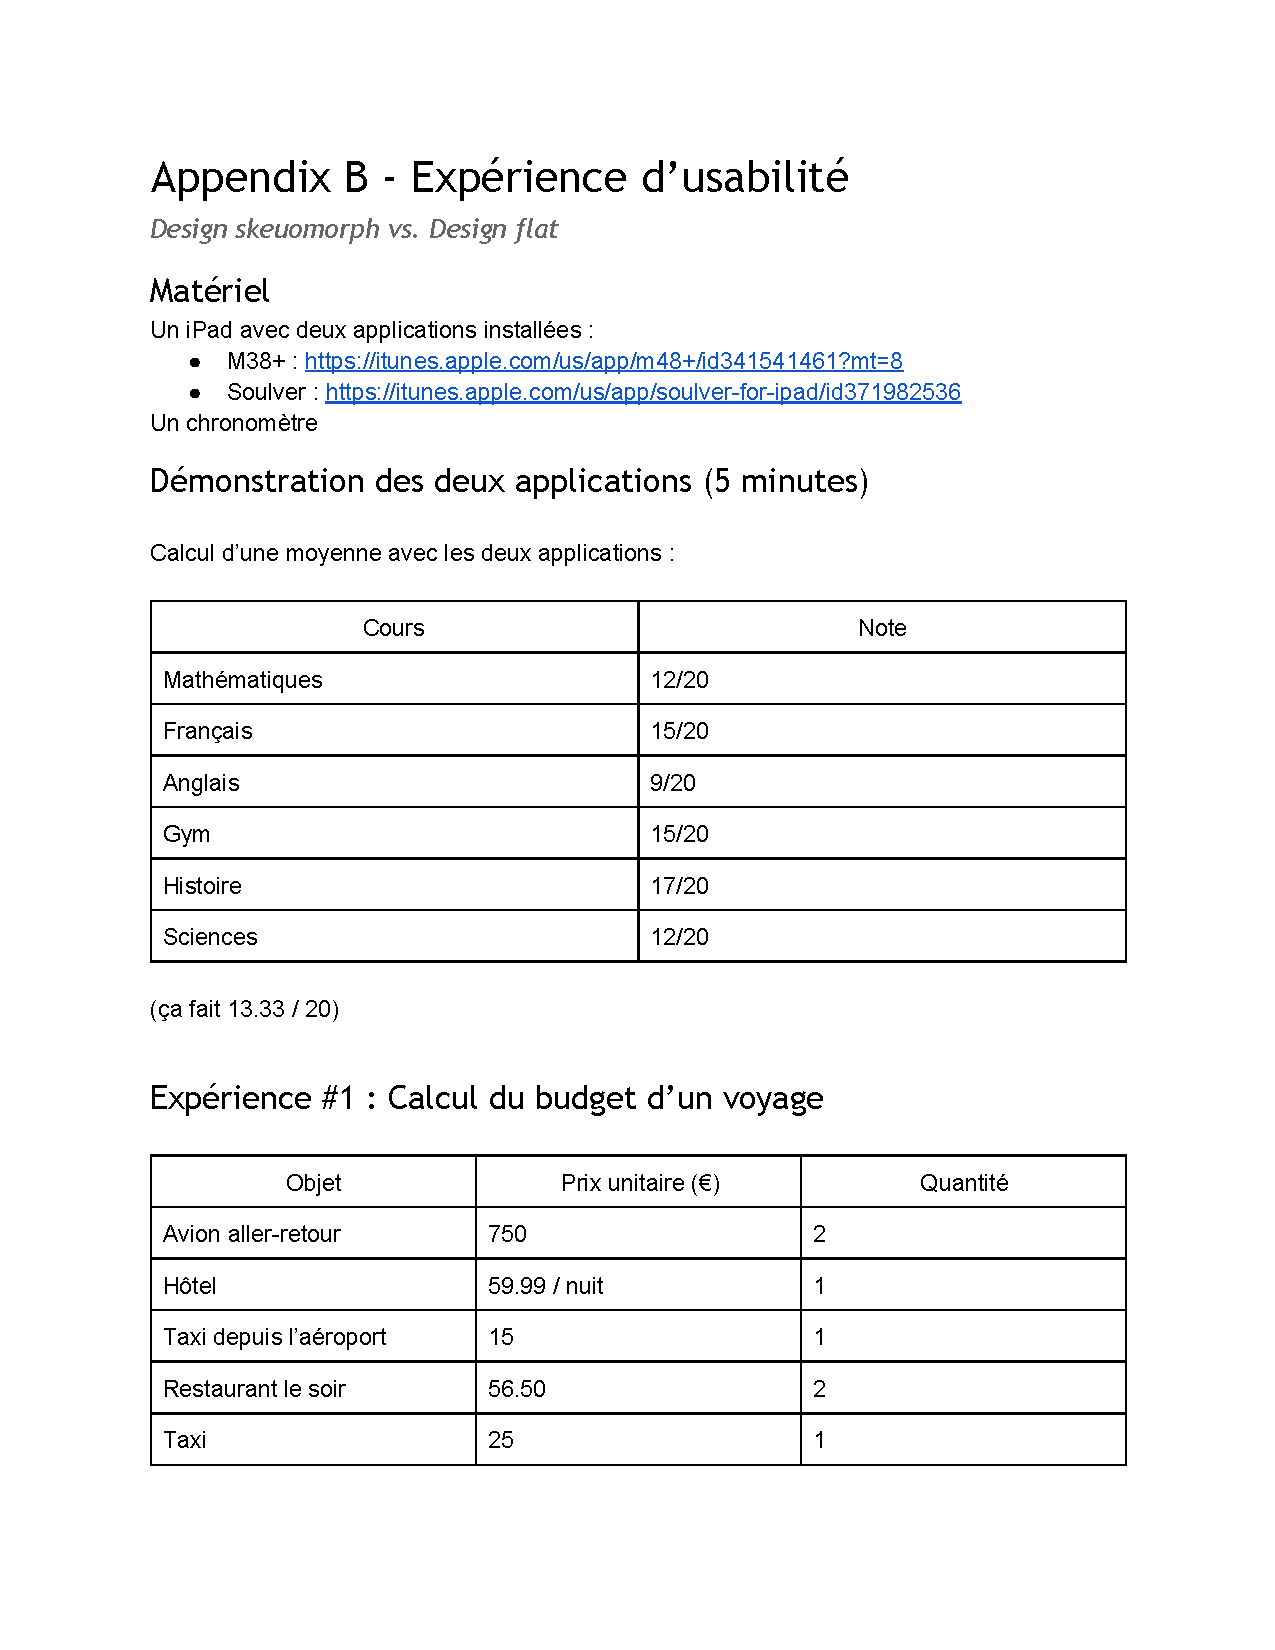
\includepdf[pages={1-2}]{fig-report/ComputersandSociety-Experiment.pdf}


\newpage
% \cite{*}
\bibliographystyle{plain}
\bibliography{bibUsability}
\end{document}
